%!TEX root=../GaugeCNNTheory.tex


\subsection{Isometry equivariance}
\label{sec:gauge_conv_isom_equiv}


\begin{SCfigure}
    \centering
    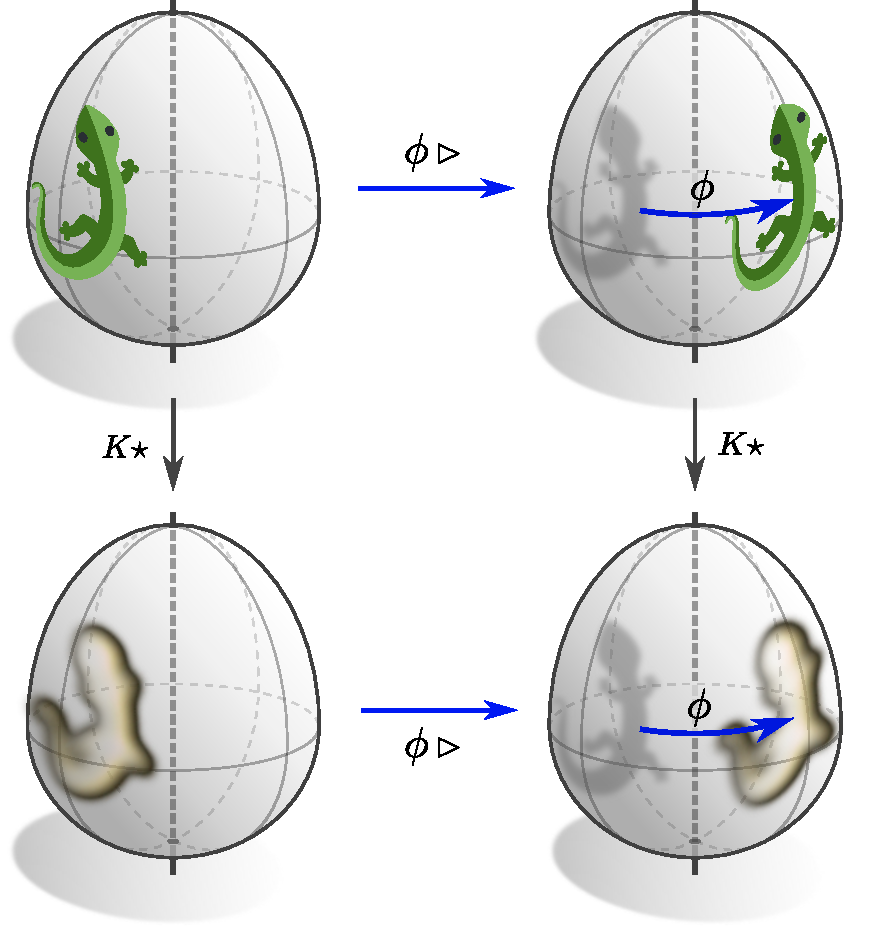
\includegraphics[width=.56\textwidth]{figures/lizard_conv_egg.pdf}
    \captionsetup{width=.89\textwidth}
    \caption[]{\small
        A network layer is said to be equivariant under isometries when it commutes with their action on feature fields.
        $\GM$-convolutions are by design equivariant w.r.t. those isometries $\phi\in \IsomGM$ that are symmetries of the $G$-structure.
        In equations, the convolution $K\star$ is equivariant under the action of an isometry $\phi$ when it satisfies the relation
        ${K \star \big( \phi\rhd\! \fin \big) = \phi\rhd\! \big(K \star \fin \big)}$
        for any choice of input field~$\fin$.
        This relation is visualized by the commutative diagram in Eq.~\eqref{cd:isometry_equivariance_conv_mapsto}, a graphical interpretation of which is shown in this figure.
        \\[1ex]
        That $\GM$-convolutions are $\IsomGM$-equivariant relies on the facts that
        1) kernels are shared over the whole manifold,
        2) isometries preserve the transporter pullback of feature fields and
        3) that $\IsomGM$ induces $G$-valued gauge transformations, which are accounted for by the kernel's $G$-steerability.
        {\\
        \color{gray}
        \scriptsize
            (Lizards adapted under the Creative Commons Attribution 4.0 International
            \href{https://github.com/twitter/twemoji/blob/gh-pages/LICENSE-GRAPHICS}{\underline{license}}
            by courtesy of Twitter.)
        }
        \\[0ex]
        }
    \label{fig:lizard_conv_egg}
\end{SCfigure}


Given that a manifold exhibits symmetries it is usually desirable that neural networks respect these symmetries, i.e. are equivariant under their action on feature fields.
$\GM$-convolutions are by design guaranteed to be $\IsomGM$-equivariant, which means that they commute with the action of isometries in $\IsomGM$ on feature fields, as visualized in Fig.~\ref{fig:lizard_conv_egg}.%
\footnote{
    Recall that an action on $\GM$-coordinate independent feature fields can only be defined for the $G$-structure preserving isometries in $\IsomGM$.
    It is therefore not even possible to define a notion of isometry equivariance for isometries that are not symmetries the $G$-structure.
    Note that this is without loss of generality since one can always choose a structure group $G=\O{d}$, for which $\IsomGM=\IsomM$ coincides with the full isometry group.
}.
Expressed in equations, the $\GM$-convolution $K\star$ is equivariant when it satisfies the relation
\begin{align}\label{eq:isometry_equivariance_conv_def_33}
    K \star \big( \phi\rhd\! \fin \big) \ =\ \phi\rhd\! \big( K \star \fin \big)
    \qquad \forall\ \ \phi\in \IsomGM
\end{align}
for any possible input field $\fin$, that is, when the following diagram commutes:
\begin{equation}\label{cd:isometry_equivariance_conv_mapsto}
\begin{tikzcd}[column sep=60pt, row sep=35, font=\normalsize]
    \fin
        \arrow[r, "\phi\,\rhd", mapsto]
        \arrow[d, "K\star"', mapsto]
    &
    \phi\,\rhd \fin
        \arrow[d, "K\star", mapsto]
    \\
    \fout
        \arrow[r, "\phi\,\rhd"', mapsto]
    &
    \phi\,\rhd \fout
\end{tikzcd}
\end{equation}


As a first step towards proving the isometry equivariance of $\GM$-convolutions, recall that they are pointwise defined as the contraction of a kernel $K$ with the transporter pullback $[\Expspfin]^A$ of the input field~$\fin$.
Since isometries preserve the Riemannian geometry of~$M$ by definition, they preserve in particular the Riemannian exponential map and Levi-Civita transporters; see Section~\ref{sec:isom_expmap_transport} and Fig.~\ref{fig:isom_exp_transport}.%
\footnote{
    More generally, whenever an alternative $G$-compatible connection is chosen to transport feature vectors, we assume this connection to be invariant under the action of $\IsomGM$; see Section~\ref{sec:isom_expmap_transport}.
    This assumption is satisfied for all models that are covered in the literature review in Part~\ref{part:literature_review}.
}
This implies that the transporter pullback of the pushforward field $\phi\rhd\fin$ at $\phi(p)$ will only differ from the transporter pullback of the original field $\fin$ at $p$ by the isometry induced gauge transformation, that is,
\begin{align}\label{eq:transporter_pullback_pushforward_field}
    \big[\mkern-2mu \Expsphip (\phi\rhd\fin) \big]^A\ =\ 
    \rhoin\big( g_\phi^{A\widetilde{A}}(p)\big) \circ \big[\mkern-2mu \Expspfin\big]^{\widetilde{A}} \circ g_\phi^{A\widetilde{A}}(p)^{-1} \,;
\end{align}
cf. Eq.~\eqref{eq:trafo_law_transporter_pullback} and, for the coordinate free formulation, Theorem~\ref{thm:transporter_pullback_isometry_action}.

Given this identity, the isometry equivariance of $\GM$-convolutions
is proven by the following simple calculation, which crucially leverages the $G$-steerability of the template kernel~$K$ to explain away the isometry induced gauge action:
\begin{align}
    \big[ K \star (\phi \rhd \fin) \big]^A (\phi(p))
    \ \overset{(1)}{=}&\ \ 
        \int_{\R^d} K(\mathscr{v})\  \big[\mkern-2mu \Expsphip (\phi\rhd\fin) \big]^A (\mathscr{v})\ d\mathscr{v} \notag \\
    \ \overset{(2)}{=}&\ \ 
        \int_{\R^d} K(\mathscr{v})\ 
        \Big[ \rhoin\pig( g_\phi^{A\widetilde{A}}(p)\pig) \big[\mkern-2mu \Expspfin\big]^{\widetilde{A}} \pig(g_\phi^{A\widetilde{A}}(p)^{-1} \mathscr{v} \pig) \Big]\ d\mathscr{v} \notag \\
    \ \overset{(3)}{=}&\ \ 
        \int_{\R^d} \Big[ K\pig( g_\phi^{A\widetilde{A}}(p)\, \tilde{\mathscr{v}}\pig)\ \rhoin\pig( g_\phi^{A\widetilde{A}}(p)\pig) \Big]\ 
        \big[\mkern-2mu \Expspfin\big]^{\widetilde{A}} (\tilde{\mathscr{v}})\ 
        \pig|\mkern-3mu\det g_\phi^{A\widetilde{A}}(p)\pig|\; d\tilde{\mathscr{v}} \notag \\
    \ \overset{(4)}{=}&\ \ 
        \int_{\R^d} \Big[\rhoout\pig( g_\phi^{A\widetilde{A}}(p)\pig)  K\big(\tilde{\mathscr{v}}\big) \Big]\ 
        \big[\mkern-2mu \Expspfin\big]^{\widetilde{A}} (\tilde{\mathscr{v}})\ d\tilde{\mathscr{v}} \notag \\
    \ \overset{(5)}{=}&\ \ 
        \rhoout\big( g_\phi^{A\widetilde{A}}(p) \big) \cdot \fout^{\widetilde{A}}(p) \notag \\
    \ \overset{(6)}{=}&\ \ 
        \big[ \phi \rhd \fout \big]^A (\phi(p)) \notag \\
    \ \overset{(7)}{=}&\ \ 
        \big[ \phi \rhd \big(K \star \fin\big) \big]^A (\phi(p))
\end{align}
The first step follows hereby from the definition of $\GM$-convolutions in Eq.~\eqref{eq:gauge_conv_coord_expression} while the second step inserted the induced gauge transformation according to Eq.~\eqref{eq:transporter_pullback_pushforward_field}.
A substitution from $\mathscr{v}$ to $\tilde{\mathscr{v}} = g_\phi^{A\widetilde{A}}(p)^{-1} \mkern1mu \mathscr{v}$ justifies step three.
In the fourth step the $G$-steerability of the template kernel, i.e. Eq.~\eqref{eq:kernel_constraint}, is applied (recall Eq.~\eqref{eq:IsomGM_coord_in_G_24}, which states that the $\IsomGM$-induced gauge transformations are $G$-valued).
What follows is that the resulting output feature vector is transformed by the induced gauge transformation.
After identifying this as the coordinate expression of the pushforward of the output field in Eq.~\eqref{eq:feature_field_trafo_in_coords}, the statement follows.
As all steps are valid for arbitrary isometries in $\IsomGM$, we see that \emph{$\GM$-convolutions are automatically equivariant w.r.t. any $G$-structure preserving isometry}.
They are \emph{not} necessarily equivariant w.r.t. general isometries in $\IsomM$, which might disrespect the $G$-structure, however, full isometry equivariance is guaranteed for orthonormal structure groups $G=\O{d}$ (or supergroups of~it).



\paragraph{Invariant kernel fields:}
A more in depth analysis of the isometry equivariance of general kernel field transforms can be found in Sections~\ref{sec:isometry_equivariance} and~\ref{sec:quotient_kernel_fields}.
The central result of this investigation is Theorem~\ref{thm:isometry_equivariant_kernel_field_trafos}, which states that \emph{the isometry equivariance of a kernel field transform implies the isometry invariance of its kernel field} and vice versa.
Fig~\ref{fig:isom_invariant_kernel_field_multiple_orbits} visualizes such an invariant kernel field, which is required to share weights over the orbits of the isometry action.
The required invariance of the kernel field is intuitively plausible since isometry equivariance certainly requires the inference of the network to be the constant on each orbit.
This abstract results implies the isometry equivariance of $\GM$-convolutions by observing that $\GM$-convolutional kernel fields -- which are determined by a single, shared template kernel -- are invariant under isometries in $\IsomGM$; see Theorem~\ref{thm:isom_equiv_GM_conv} and Fig.~\ref{fig:intro_invariant_kernel_fields_plane}.
The template kernel's $G$-steerability accounts thereby for the invariance of kernels under the action of stabilizer subgroups of the isometry group.



\paragraph{Homogeneous spaces:}
While the demand for isometry equivariance requires kernels to be shared over orbits of the isometry group, it does in general not require convolutional weight sharing over the whole manifold.
An important exception is the case of manifolds that are \emph{homogeneous spaces} of their isometry group, like for instance $\R^d$ or the sphere $S^2$.
By definition, the isometry action is on such spaces transitive, that is, there exists only one single orbit.
Consequently, there will only be one independent kernel, which is via the action of the isometry group being shared over the whole space.
Theorem~\ref{thm:GM_conv_homogeneous_equivalence} in Section~\ref{sec:quotient_kernel_fields} proves that \emph{isometry equivariant kernel field transforms on homogeneous spaces are necessarily coordinate independent convolutions}.
This observation establishes a formal link between our theory and prior work on convolutional networks on homogeneous spaces
by~\citet{Kondor2018-GENERAL}, \citet{Cohen2019-generaltheory} and~\citet{bekkers2020bspline},
who are defining convolutions via their equivariance w.r.t. global symmetries of the underlying space.






\paragraph{Diffeomorphism equivariance:}
The reader might wonder whether it is possible to make our coordinate independent CNNs fully diffeomorphism equivariant.
As one can easily see, the pointwise operations from Section~\ref{sec:pointwise_operations}, i.e. \onexones, biases and nonlinearities, are already diffeomorphism equivariant.
Specifically, let
\begin{align}\label{eq:DiffGM_def_part1}
    \DiffGM\ :=\ \pig\{ \phi \in \Diff(M) \ \pig|\ 
    \big[\phi_*(e_i)\big]_{i=1}^d \in \GM \quad \forall\ [e_i]_{i=1}^d \in \GM \pig\} \,\ \leq\ \Diff(M)
\end{align}
be the subgroup of $G$-structure preserving diffeomorphisms, i.e. the analog to Eq.~\eqref{eq:IsomGM_def_24} without the requirement on~$\phi$ to be an isometry.
Similarly to Eq.~\eqref{eq:IsomGM_coord_in_G_24} and Theorem~\ref{thm:isom_GM_in_coords}, the coordinate expressions (induced gauge transformations) of $G$-structure preserving diffeomorphisms are guaranteed to take values in $G$, that is,
\begin{align}
    \phi \in \DiffGM \quad \Longleftrightarrow \quad g_\phi^{A\widetilde{A}}(p) \in G\ \ \ \forall\ p \mkern-1mu\in\mkern-2mu M \,.
\end{align}
The $G$-equivariance of the shared pointwise template functions will guarantee that they commute with these $\DiffGM$-induced gauge transformations -- and therefore with the active diffeomorphism action itself.


$\GM$-convolutions with spatially extended kernels, on the other hand, are in general \emph{not} equivariant w.r.t. diffeomorphisms.
The reason for this is that the transporter pullback $\Expspf$ relies on exponential maps, which are inherently Riemannian constructions that do not commute with diffeomorphisms.
However, as the kernels are $G$-steerable, $\DiffGM$-equivariance should nonetheless hold in the limit of the kernel support going to zero.
Given that convolution kernels are in typical deep learning applications quite small, diffeomorphism equivariance should in practice hold approximately.



\paragraph{Affine equivariance:}
Euclidean spaces constitute a special case since they allow for $\GM$-convolutions that are equivariant under the action of \emph{affine groups}~$\Aff(G)$.
That this is the case relies on the fact that the exponential map commutes on Euclidean spaces not only with the action of isometries but more generally with affine transformations.
The affine group equivariance of Euclidean $\GM$-convolutions is proven in Section~\ref{sec:euclidean_affine_equiv}.
